\section{Arctic Home in the Vedas}

\begin{quotex}
From the dead sun springs a daughter more beautiful than her sire, and mankind starts afresh from the life-raiser and his bride-Life. 

\end{quotex}

In which we briefly outline the idea of cosmic cycles, and illustrate them initially in the revelation of the originary Hyperborean source of the Vedas. This is then extended to Traditions following the Vedas. Finally, there is some speculation on the future course of the West. The foundation is the book \textit{The Arctic Home in the Vedas} by \textbf{Bal Tilak}.

\paragraph{Cosmic Cycles}
Since a more complete exposition can be found in Rene Guenon's writings, from whom these notes are taken, and elsewhere, we provide here just the most basic outline.

\textbf{Cycle}: represents the process of development of some state of manifestation

\textbf{Minor cycle}: one of the more or less restricted and specialized modalities of that state

Since the \textbf{Law of Correspondence} links all things in universal Existence, is necessarily and always a certain analogy, either among different cycles of the same order or among the principal cycles and their secondary divisions

\textbf{Kalpa}: total development of a world. One cannot speak literally about its duration so that duration has a purely symbolic value. Perhaps not in our world because time is one of its determining conditions.

\textbf{Manu}: there are 14 Manus, each ruling over a Manvantara. There are two septenary series. The first septenary is that of descent, or devolution, and includes ours. The second is ascent or evolution.

\textbf{Manvantaras}: cycles have a character that is both cosmic and historical, they concern terrestrial humanity, also linked to events occurring outside the history of humanity. There is a correlation between the cosmic and human orders. This means, for example, that events in the human realm correspond to events in the celestial spheres.

These relate to the 7 \textbf{svargas} and 7 \textbf{patalas} which represent states respectively higher and lower than the human state. By correspondence, these can be related to the 14 manus.

\begin{wrapfigure}{rt}{.3\textwidth}
 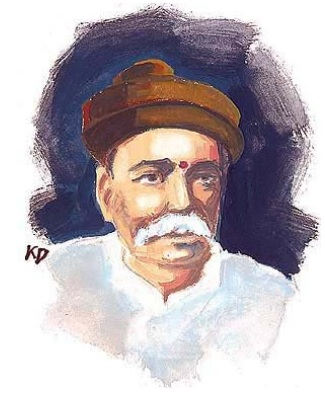
\includegraphics[scale=.5]{a20200723ArcticHomeintheVedas-img001.jpg} 
 \caption{Bal Tilak}
\end{wrapfigure} 

A Mantavara is subdivided into 4 \textbf{yugas}. We are allegedly in the last yuga, the Kali Yuga. The starting date and exact duration are not known, according to Rene Guenon.

There are 7 \textbf{Dvipas} or regions into which our world is divided. They are represented as islands or continents, but not parts of present-day earth. They may also refer to planetary spheres.

These ages, states, and regions also have symbolic meanings, since there is a sacred geography as well as a profane geography. Henry Corbin discusses this topic in his books, and it is also confirmed by Rene Guenon:

\begin{quotex}
There is also a symbolical geography; indeed, in this connection, there is a very significant correspondence between the domination of the West and the end of a cycle, for the West is the place where the sun sets. 

\end{quotex}
Thus, when he mentions the distinction between Eastern and Western understanding, this is no way simply a geographic distinction; i.e., there is no ``magic dirt" in the East. Guenon amplifies the idea:

\begin{quotex}
To the extent that a man `Westernizes' himself, whatever may be his race or country, to that extent he ceases to be an Easterner spiritually and intellectually. 

\end{quotex}
The converse is also true. Unfortunately, this is too often overlooked so there are some who fantasize about going east to find an ``initiatic centre" or give up entirely. Often, they justify this decision because of the ``corruption" they see in the Church hierarchy, as though India and Egypt are free of such corruption. These masters of ignorance have a loud presence on social media. The truth is that real initiates like Savonarola, Boccaccio, and Dante were complaining about corruption in the Church a thousand years ago. (See Canto XXI, \emph{Paradiso}, for example.)

How, then, could Dante describe his spiritual journey? His passage through Purgatory and Heaven are descriptions through the higher and lower stages. Guenon provides us with the general idea, but we need to get the details from others who have made the trip.

\paragraph{Hyperborean Migration}
The idea of a migration of a branch of the Borean race from a polar region to India has been a mainstay in esoteric literature. That is now considered outré and dismissed as the ``Aryan Invasion Theory". Times change. Bal Tilak, the author of The Arctic Home in the Vedas, was a Hindu nationalist and considered himself to be Aryan; so, it is not a Nazi fantasy. Perhaps there is no genetic, archaeological, or documentary proof. Nevertheless, as Georges Dumezil documented, there is still the trifunctional social organisation from Scandinavia, across Europe, to India that needs to be explained. Moreover, there is similarity in the mythologies of the various Indo-European people.

In any case, it may be best to regard Hyperborea as transcendent geography or one of the seven Dvipas. That is how the Greeks understood it, since only the gods could visit it. Apollo would arrive there by a swan.

Nevertheless, Tilak probes through the Vedas looking for clues for an actual migration several millennia ago. In particular, he sees astronomical facts that match the experience of a those living in a land close to the North Pole. For example, the original Roman calendar had 10 months, ending in December. That is because it would be followed by two months of darkness during which days could not be counted. It continues in that vein, relying as much on Western scholars as on the Vedas themselves.

Sometimes it gets tedious, much like exegesis on Genesis; is a ``day" 24 hours or does it refer to an age? Nevertheless, it is worth the trouble because of the vast amount of information in it.

The Vedas are eternal and without beginning. However, we owe the textual version to the seven Rishis who could ``see" the vedas from the beginning of the Kalpa. A deluge had destroyed the Vedas at the end of the previous Kalpa. Tilak's method is to juxtapose the Theological view in the Vedas with a corresponding Historico-scientific view gathered from external and profane sources. He also relies on comparative mythology relating Celtic, Greek, Roman, and Egyptian myths to corroborate the Vedic myths. Most importantly, Tilak regards the Zend Avesta, the sacred text of the Zoroastrians, as authoritative.

\paragraph{The Divine Word}
Since, this is an introduction, we can only point out some highlights; maybe someday we can do a more exhaustive review. This is an important point:

\begin{quotex}
Vedic names and forms of species are eternal, and it is by remembering these that the world is created by Brahmâ at the beginning of each Kalpa. The Veda is, therefore, the original WORD, the source from which everything else in the world emanated, and as such it cannot but be eternal. 

\end{quotex}
Tilak points out that this doctrine is tantamount to the notion of the divine \emph{Logos} of the Alexandrian school.

The duration of the various ages or yugas were in dispute. For example, by an early reckoning, the Kali Yuga would have ended soon after the birth of Christ. Although they knew nothing of that event, the authors of the Puranas in the first centuries AD, refused to believe the Kali Yuga had ended. Hence they extended the duration from 1000 human years to divine years (360 human years). Tilak points to similar artifices to fudge the dates for various purposes. The alternative is to assume that the Christian Era represented the end of the Kali Yuga and the beginning of an ascent.

The point is that the authors preferred to understand the ages by their qualities, not merely as the passage of quantitative time. Also, the original timeframes were much shorter than the fantastical extended duration of the ages that get passed around today.

\paragraph{Excursus on Method}
Tilak is very thorough, although the text points out the difficulty of fully understanding the Vedas in all cases. Both Evola and Guenon accepted Tilak's thesis; the latter actually thought very highly of Tilak. Guenon reveals some contradictions in his doctrines that require explanation. For example,

\begin{itemize}
\item Guenon claims Tilak was a non-Westernized Hindu. \textbf{FACT}: Tilak was quite familiar with European science, history, and mythology. Moreover, he had deep respect for the German Indologist, Max Müller. 
\item Guenon tediously rails against ``profane" science, history, philosophy, etc. \textbf{FACT}: Tilak relied heavily on those ``profane" fields of study to fortify his thesis. 
\item Guenon hates Vivekananda, but loves Tilak. \textbf{FACT}: Vivekananda was esteemed by not just Tilak, but even Hindus in India to this day. 
\end{itemize}
The point is that it is a mistake to disdain ``profane" scholarship when it might be helpful. By the Law of Correspondences, science and metaphysics should not be in conflict since they deal with different levels of existence. Guenon has done us a great service by his explanations of metaphysics and symbolism, by his deep comparisons of different traditions, and by expanding our understanding to include the full range of authentic human spirituality. There is no ``Guenonian doctrine" per se, since he is just rephrasing the doctrines of traditions that pre-existed him.

At the end of the day, Guenon does not judge Tradition; Tradition judges Guenon. That is lawful, not a negative judgment.

\paragraph{Traditional Forms}
It is one thing to mention the possibility of different stages/regions/states, etc., and quite another to fill in the details. That would perhaps require another Rishi, not for a new revelation, but rather for a deeper understanding. Tilak gives us some clues about how the different stages of Tradition might look.

The Letters to the Seven Churches in the Book of Revelation represent the seven stages of the development of Tradition. The following list represents Valentin Tomberg's understanding of the stages. This list is remarkably consistent with Tilak's exposition of the Vedas, with some speculation about the future.

\begin{enumerate}
\item \textbf{Ephesus}: The old Indian (Vedic) culture. This is primal revelation given to the Rishis in India. 
\item \textbf{Smyrna}: The old Persian (Zoroastrian) culture. The Zend Avesta also retained a memory of the Hyperborean revelation. 
\item \textbf{Pergamos}: The Chaldean-Egyptian (Hermetic) culture. This is based on the revelation of the Logos to the Alexandrian school. 
\item \textbf{Thyatira}: The Greco-Roman (pagan) culture. Although the Greeks retained some memory of Hyperborea, much came through Egypt. The Greeks had the same understanding of ``name and form" from Vedic metaphysics, despite the different emphases of Plato and Aristotle. 
\item \textbf{Sardis}: The Anglo-Germanic (Christian) culture. The Christian religion transformed Europe with a deeper revelation. Building on the Vedas and Hermetics, it understood the Logos as not just the creator, but also as equal to God as well as saviour and judge. Christianity got its philosophy from the Greeks and its Theology was enriched by the Alexandrian school as Vladimir Solovyov pointed out. 
\item \textbf{Philadelphia:} The Slavic-Russian (also Christian) culture. The Slavic nations should be the preservers of Tradition. We shall see how that plays out. 
\item \textbf{Laodicea:} The American, i.e. Western Hemisphere, (future) culture. North and South America will look quite different in the future. More cannot be said at this time. 
\end{enumerate}
There are three churches of the past, two of the present, and two of the future. But do not take the history and geography too literally, for they represent streams that are always active in us.



\flrightit{Posted on 2020-07-23 by Cologero }

\begin{center}* * *\end{center}

\begin{footnotesize}\begin{sffamily}



\texttt{Christopher on 2020-07-23 at 15:48 said: }

``Guenon tediously rails against ``profane" science, history, philosophy, etc. FACT: Tilak relied heavily on those ``profane" fields of study to fortify his thesis."

While I agree generally with the tediousness of Guénon in this regard, I don't believe it to be a contradiction. Guénon has, at various times, cited archaeological findings (his article on La triple enceinte druidique comes to mind) and defended the potential use of profane archaeology, even while criticizing its current usage. In his article on the Place de la tradition atlantéene dans le Manvantara (Le Voile d'Isis, August–September 1931), he wrote:

« On ne saurait être trop prudent quand il s'agit de civilisations entièrement disparues, et ce ne sont certes pas les tentatives de reconstitution auxquelles se livrent les archéologues profanes qui sont susceptibles d'.claircir la question ; mais il n'en est pas moins vrai que beaucoup de vestiges d'un passé oublié sortent de terre à notre époque, et ce ne peut être sans raison. Sans risquer la moindre prédiction sur ce qui pourra résulter de ces découvertes, dont ceux qui les font sont généralement incapables de soupçonner la portée possible, il faut certainement voir là un «signe des temps» : tout ne doit-il pas se retrouver à la fin du Manvantara, pour servir de point de départ à l'.laboration du cycle futur ? »

``One cannot be too cautious when dealing with civilizations that have completely disappeared, and it is certainly not the attempts at reconstitution made by profane archaeologists that are likely to shed light on the matter, but it is no less true that many vestiges of a forgotten past are coming out of the ground in our time, and this cannot be without reason. Without risking the slightest prediction about what may result from these discoveries, whose possible significance is generally not suspected by those who make these discoveries, we must certainly see this as a `sign of the times.' Should not everything be found at the end of the Manvantara, to serve as a starting point for the elaboration of the future cycle?"


\hfill

\texttt{Logres on 2020-08-05 at 23:20 said: }

``The alternative is to assume that the Christian Era represented the end of the Kali Yuga and the beginning of an ascent." Rudolf Steiner seems to have come to this conclusion, and much of what you review in Tilak resonates with what I've been able to glean there.

\url{https://martyrion.blogspot.com/2015/11/jesus-of-gospel-of-matthew.html}

\begin{quotex}
It is not only in man that a change has taken place; everything in Nature, everything on Earth, was also changed at the descent of man. It was therefore not enough for man simply to say: All this is maya, is illusion — let us raise ourselves to the spiritual world! We shall then certainly have changed ourselves, but not all that has become changed in the world around us.' So the Iranian did not say: `Around me is maya on every side — I will rise above this maya, will overcome it in myself, and so attain to spiritual worlds.' No, he said: `Man belongs to the world around him; he is but a part of it. Therefore if that which is divine in him, and which descended with him from spiritual heights, is to be changed, then not only man must be changed back again, but everything that surrounds him must also be changed back to what it was.' This feeling gave this people a special impulse to enter energetically into the task of transforming and changing the world. While the Indian said: `The world has changed, deteriorated; what we now behold is maya,' the people of the north said: `Certainly the world has come down, but we must so change it that it is made into something spiritual once more!'

\end{quotex}
The idea being, that by the very fact of the Fall, lower matter is redeemed by the presence of the ruined image of God, and is now ``involved". This translates into understanding ``struggles between cultures", although not entirely literally. For instance, Steiner cites the Turanian struggle here:

\begin{quotex}
The Turanians in the north toward Siberia, who had inherited a lower astral clairvoyance, had no desire to establish external civilization, and their passive disposition, influenced by many priests who practiced magic, led them frequently to occupy themselves with lower magic, and even black magic. To the south, the Iranians, with an inclination to influence the sense world by their human spiritual force, were working in a primitive way at the beginnings of civilization.

This is the great contrast between Iranians and Turanians. These facts are expressed in a beautiful myth: the legend of Djemjid. 

\end{quotex}
Thank you for the note on the Seven Churches, and indeed, the entire article.


\end{sffamily}\end{footnotesize}
